% 小时百科图标
% 小时百科|图标|logo|正态分布

\begin{issues}
\issueTODO
\end{issues}

小时百科的图标是由 4 条丝带组成 3D 立体图, 从数学上来看, 每条丝带的形状分别是一个高斯分布(正态分布)\upref{GausPD}; 物理上, 四条丝带可以分别看作量子力学中自由粒子的高斯波函数随时间演化\upref{GausWP}; 艺术上, 可以寓意为海浪.

目前图标分为立体版本(\autoref{xwLogo_fig2} )和扁平化版本(\autoref{xwLogo_fig1} ).

\begin{figure}[ht]
\centering
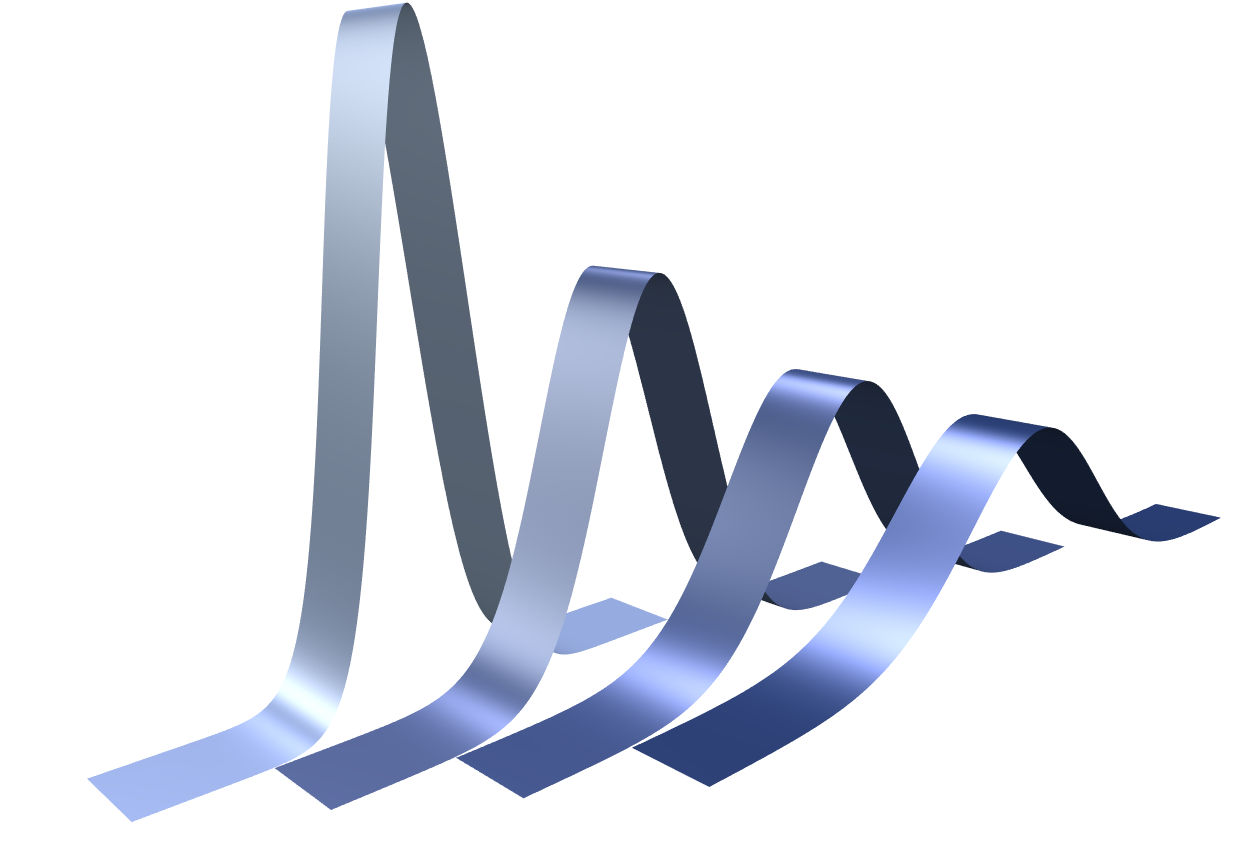
\includegraphics[width=8.3cm]{./figures/xwLogo_2.png}
\caption{立体图标, 完成于 2014 年 10 月} \label{xwLogo_fig2}
\end{figure}

\begin{figure}[ht]
\centering

\includegraphics[width=8cm]{./figures/xwLogo_1.pdf}
\caption{扁平化图标, 完成于 2020 年 9 月} \label{xwLogo_fig1}
\end{figure}

\subsection{参数}
图标使用透视投影\upref{proj3D}, 每个带的长宽高分别在\autoref{xwLogo_fig3} 中标出.
\begin{figure}[ht]
\centering
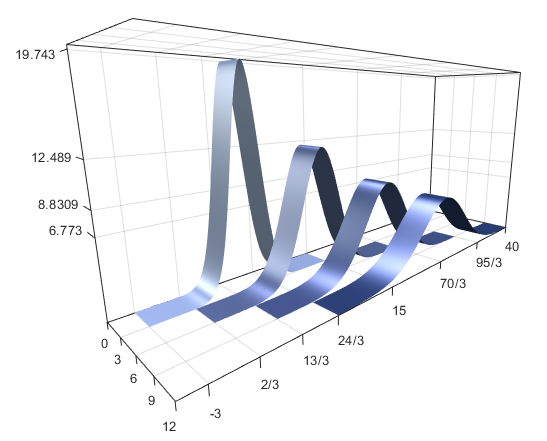
\includegraphics[width=12cm]{./figures/xwLogo_3.png}
\caption{图标参数} \label{xwLogo_fig3}
\end{figure}
\addTODO{量子力学参数, 相机参数, 光源材质参数, Matlab 代码}
